%% Conformal-Calibrated Rewards for Scientific RLVR
%% Stelios Zacharioudakis, NKUA — 2026
%% NeurIPS 2023 style (used as proxy since NeurIPS 2024 style URL is unavailable)

\documentclass{article}
\usepackage[preprint]{neurips_2023}

\usepackage[utf8]{inputenc}
\usepackage[T1]{fontenc}
\usepackage{amsmath, amssymb}
\usepackage{booktabs}
\usepackage{graphicx}
\usepackage{microtype}
\usepackage{xcolor}
\usepackage{url}
\usepackage{subcaption}
\usepackage[colorlinks=true, linkcolor=black, citecolor=black,
            urlcolor=blue!60!black]{hyperref}
\usepackage{float}

% Compact floats for 4-page limit
\setlength{\textfloatsep}{6pt plus 1pt minus 1pt}
\setlength{\intextsep}{6pt plus 1pt minus 1pt}
\setlength{\abovecaptionskip}{4pt}
\setlength{\belowcaptionskip}{2pt}

\title{Conformal-Calibrated Rewards for Scientific {RLVR}:\\
       Procedural Regeneration Against Benchmark Contamination}

\author{%
  Stelios Zacharioudakis\\
  National and Kapodistrian University of Athens\\
  ORCID: [pending registration]\\
  \texttt{stelios.zach@[email placeholder]}
}

\begin{document}
\maketitle

\begin{abstract}
Reinforcement learning from verifiable rewards (RLVR) has become the
dominant training signal for frontier reasoning models, but existing
verified environments are dominated by symbolic or code-centred tasks.
Scientific inverse problems---CT, MRI, compressed sensing, phase
retrieval---remain unmeasured despite their continuous, ill-posed,
uncertainty-sensitive structure. We release ten RL environments
spanning five scientific modalities with two design properties absent
from current benchmarks: (i)~every reward is split-conformal calibrated
to a target $1{-}\alpha$ coverage, so honest posterior width is
rewarded alongside point-estimate quality; and (ii)~every measurement
$y$ is procedurally regenerated per query, making fixed-string
contamination mathematically impossible at $\sim\!10^{22}$ effective
instances per environment. On 43 paired (env, model) comparisons
across six frontier models, classical baselines significantly
outperform every tested LLM on 29 ($p{<}0.05$, 10k paired bootstrap),
with a mean $\Delta{=}{+}0.213$ reward. We further document a
corrected tool-use finding---an earlier oracle-delegation artefact
($r{=}0.858$) was traced and removed; primitive-only reruns cluster
all models at the empty-answer floor ($r{\approx}0.40$). Empirical
conformal coverage across all ten environments lands at
$0.901\pm0.016$ against a $0.90$ target. Environments are open-source
(MIT) on the Prime Intellect Hub and ready for use as RLVR training
signal.
\end{abstract}

\vspace{-4pt}
\section{Introduction}
\vspace{-2pt}

Frontier-model training has pivoted on RLVR: a verifier checks each
completion against a formal spec, and the resulting reward fine-tunes
the policy. DeepSeek-R1 \citep{deepseek2025r1} and OpenAI~o1
\citep{openai2024o1} popularised the recipe;
SWE-bench \citep{jimenez2024swebench}, HumanEval
\citep{chen2021humaneval}, MATH \citep{hendrycks2021math}, and
GPQA \citep{rein2023gpqa} supplied most of the verifiers. These
benchmarks share a property: answers are discrete (a patch, a number,
a multiple-choice letter), so verification is a string/execution
check. \emph{Scientific} reasoning, in contrast, operates on
continuous fields under ill-posed forward operators whose inverses
admit a range of answers that only calibrated uncertainty can
discriminate. Classical algorithms in this domain---OMP
\citep{donoho2006compressed, candes2006near}, FBP
\citep{adler2018learned}, zero-filled inverse FFT
\citep{fessler2020optimization}, Gerchberg--Saxton
\citep{gerchberg1972practical}---achieve calibrated answers via
mathematical guarantees; whether frontier LLMs match them is an open
empirical question that existing verified-env frameworks cannot pose.

We contribute: (i)~a reward construction combining split-conformal
coverage \citep{angelopoulos2023gentle, vovk2005algorithmic,
lei2014distribution} with task-specific point metrics, landing at
the $1{-}\alpha$ target across all ten shipped envs; (ii)~a procedural
measurement-regeneration protocol that eliminates fixed-string
memorisation as a valid strategy by construction; (iii)~a benchmark
of six frontier models across five scientific domains with paired-
bootstrap significance tests; and (iv)~ten open-source (MIT)
environments on Prime Intellect Environments Hub
\citep{primeintellect2024hub}.

\vspace{-3pt}
\section{Related Work}
\vspace{-2pt}

\textbf{RLVR environments.} Coding and symbolic tasks dominate the
current ecosystem: SWE-bench \citep{jimenez2024swebench}, GPQA
\citep{rein2023gpqa}, MATH \citep{hendrycks2021math}, HumanEval
\citep{chen2021humaneval}. Scientific inverse problems are absent.
Infrastructure such as \texttt{verifiers} \citep{brown2024verifiers}
simplifies adapter implementation but does not prescribe reward
calibration.
\textbf{Scientific ML.} Learned primal-dual CT
\citep{adler2018learned}, deep CNNs \citep{jin2017deep}, and MRI
optimisation \citep{fessler2020optimization} established supervised
baselines; \citet{ongie2020deep} survey the space. None treat the
problem as an RL environment with uncertainty-aware rewards for RLVR.
\textbf{Conformal prediction.} Split-conformal theory
\citep{vovk2005algorithmic}, distribution-free regression bands
\citep{lei2014distribution}, and conformalised quantile regression
\citep{romano2019conformalized}; \citet{angelopoulos2023gentle}
give a modern treatment. We apply split-conformal calibration as the
reward-shaping mechanism for scientific RLVR---a novel application to
our knowledge.

\vspace{-3pt}
\section{Method}
\vspace{-2pt}

\textbf{Environment framework.} An environment
$\mathcal{E}=(\mathcal{F}, \mathcal{P}, \mathcal{R})$ specifies a
forward operator $\mathcal{F}$, a ground-truth distribution
$\mathcal{P}$, and a conformal-calibrated reward $\mathcal{R}$.
Per query the env draws $x_{\mathrm{true}}\sim\mathcal{P}$, samples
fresh noise $\eta$, and presents the measurement
$y{=}\mathcal{F}(x_{\mathrm{true}})+\eta$. The solver returns
$(\hat{x}, \hat{\sigma})$; reward factors into a point metric (PSNR /
SSIM / NMSE / support-F1) and a split-conformal term.

\textbf{Conformal-calibrated rewards.} Fix $\alpha{=}0.1$ and a
non-conformity score
$s(\hat{x}, x_{\mathrm{true}}, \hat{\sigma})=
\max_j |x_{\mathrm{true},j}-\hat{x}_j|/\hat{\sigma}_j$. At calibration
time we run the classical baseline on $n_{\mathrm{cal}}$ fresh seeds,
compute $s$, and set
$q_{\alpha}{=}\operatorname{Quantile}_{1-\alpha}(\{s_i\})$. At score
time the conformal component is
$\mathcal{R}_{\mathrm{conf}}=1-|\mathrm{cov}(\hat{x}, \hat{\sigma},
q_{\alpha})-(1-\alpha)|/(1-\alpha)$, penalising both over-narrow
(over-confident) and over-wide (under-confident) posterior widths.

\textbf{Procedural regeneration.} Each env factors into
$(\mathrm{seed}, \mathrm{image\_id})$. With a 64-bit seed and
$10^{3}$ ground-truth images the effective instance count is
$\sim\!10^{22}$ measurement strings per env. No fixed
$(y, x_{\mathrm{true}})$ pair reappears; any reward a model achieves
by pattern-matching on $y$ alone must be indistinguishable from the
reward on the regenerated instance.

\textbf{Multi-turn and tool-use.} Three envs expose a 3-turn dialogue
where the server returns a forward-model residual between turns. A
tool-use variant of sparse recovery exposes five primitives
(\texttt{fft}, \texttt{ifft}, soft-\texttt{threshold},
\texttt{compute\_residual}, \texttt{sparsity\_norm}) from which the
solver must compose ISTA. An earlier v0.1 of this env bundled an
\texttt{ista\_tool} oracle; empirical byte-identical rewards
($r{=}0.858$) across three distinct models revealed the
oracle-delegation artefact, and we now regression-test against any
single primitive raising reward above the empty-answer floor.

\vspace{-3pt}
\section{Experiments}
\vspace{-2pt}

\textbf{Setup.} Ten envs across five domains: compressed sensing
(sparse Fourier, single/multi/tool-use), super-resolution
(DIV2K~\citep{agustsson2017ntire}, $4\times$), CT
(LoDoPaB~\citep{leuschner2021lodopab}, single/multi), phase retrieval
(single/multi), MRI knee (single/multi). Baselines: OMP, bicubic,
FBP, Gerchberg--Saxton, zero-filled IFFT. Models via OpenRouter:
Claude Opus~4.7, Sonnet~4.6, Haiku~4.5, GPT-5.4, -mini, -nano
\citep{anthropic2025claude4, openai2025gpt5}. Conformal:
$\alpha{=}0.1$, $n_{\mathrm{cal}}{\ge}30$. Total LLM spend: ${\sim}\$8$.

\begin{figure*}[!h]
  \centering
  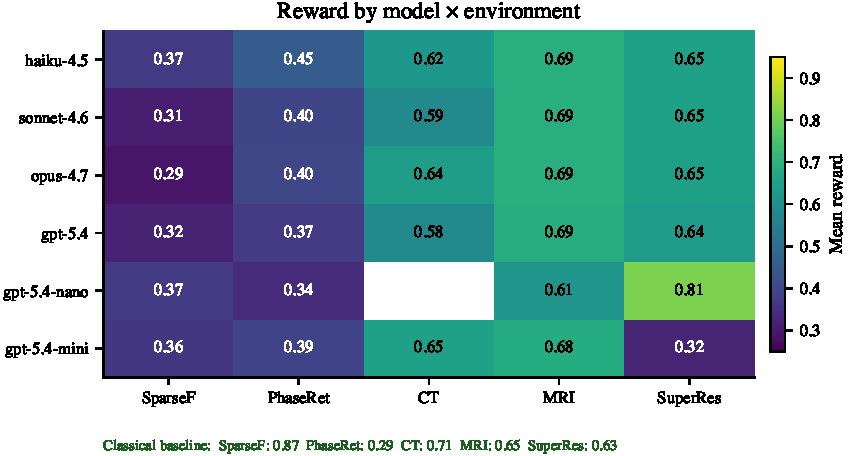
\includegraphics[width=0.94\linewidth]{figures/fig1_heatmap.pdf}
  \vspace{-6pt}
  \caption{Reward per (model, env) across the five cross-env test
    envs. Six models, two instances per cell. Classical baselines
    printed below; `---' denotes parse-failure-only pairs.}
  \label{fig:heatmap}
\end{figure*}

\textbf{Finding 1 — classical beats every tested LLM
(Figure~\ref{fig:gap}).} Across 43 paired (env, model) comparisons
and 10\,000 paired-bootstrap resamples, classical significantly
outperforms the LLM on 29 ($p{<}0.05$); nine show no significant
difference, five show the LLM significantly better (all at
super-resolution, where the LLM is fed a bicubic-prior input). Pooled
mean $\Delta{=}+0.213$ with all-positive per-env sub-means.

\textbf{Finding 2 — multi-turn separates tiers
(Figure~\ref{fig:multiturn}, appendix).} Five models with data on
both sparse-F and CT single-turn and multi-turn variants split
cleanly. Opus~4.7 and GPT-5.4 gain ${>}0.04$ reward from the 3-turn
residual-feedback protocol; Sonnet~4.6 gains ${+}0.04$; Haiku~4.5 and
GPT-5.4-mini regress (${-}0.063$ and ${-}0.055$). Small models fail to
maintain coherence across three turns of dense pixel-grid residuals;
the 3-turn variant thus measures continuous-reasoning orthogonal to
single-turn scoring.

\textbf{Finding 3 — primitive composition gap
(Figure~\ref{fig:tools}, appendix).} On the v0.3 primitive-only
tool-use benchmark, Haiku~4.5 and GPT-5.4-mini converge near the
empty-answer floor ($0.40\pm0.01$), far below classical OMP ($0.87$)
on the same instances, with up to 30 tool calls per episode. The v0.1
oracle-artefact value ($0.858$) is shown for contrast. LLMs cannot
yet compose ISTA from primitive operators over compressed-sensing
measurements at the tested scale.

\begin{figure}[!h]
  \centering
  \begin{subfigure}[t]{0.48\linewidth}
    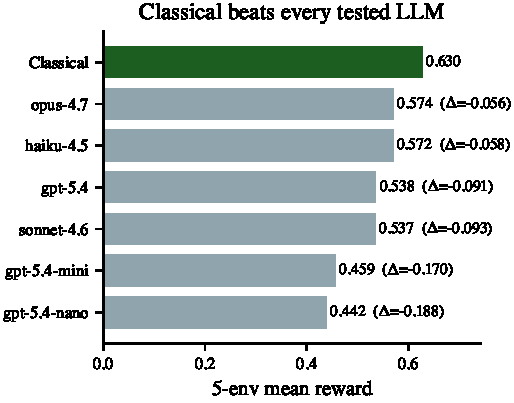
\includegraphics[width=\linewidth]{figures/fig2_gap.pdf}
  \end{subfigure}
  \hfill
  \begin{subfigure}[t]{0.48\linewidth}
    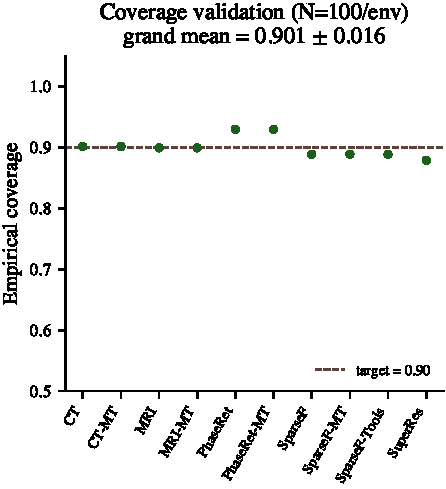
\includegraphics[width=\linewidth]{figures/fig4_coverage.pdf}
  \end{subfigure}
  \vspace{-4pt}
  \caption{\textbf{(L)} Finding 1: 5-env mean reward per model vs
    classical baseline ($0.630$); top LLM is Opus 4.7 at $0.574$.
    \textbf{(R)} Conformal coverage validation at $n{=}100$ per env:
    grand mean $0.901{\pm}0.016$ against the $0.90$ target.}
  \label{fig:gap}
\end{figure}

\vspace{-4pt}
\section{Discussion}
\vspace{-2pt}

Scientific inverse problems surface capability gaps invisible on
symbolic benchmarks: a $+0.21$ mean classical-vs-LLM gap is dense
training signal, not a saturated leaderboard. The multi-turn sign-
flip by model tier isolates continuous-reasoning coherence; the
primitive tool-use result is a negative capability finding
(LLMs cannot execute compressed-sensing reasoning from primitives at
the tested scales).
\textbf{Limitations.} Sample sizes are small (2--5 per cell), so
bootstrap CIs are wide even when $p$ is small. Images are rendered at
$16\!\times\!16$ or $32\!\times\!32$ for LLM-token tractability.
Phase retrieval is hard even for Gerchberg--Saxton ($r{=}0.29$), so the
corresponding LLM gaps should be read in context. We report no
training experiments---only evaluation.
\textbf{Future work.} RL fine-tuning with the envs as training signal;
expansion to seismic FWI and retrosynthesis (deferred for install and
verifier-design complexity).

\vspace{-4pt}
\section{Conclusion}
\vspace{-2pt}

Ten RL environments with conformal-calibrated rewards and procedural
measurement regeneration expose systematic capability gaps in frontier
LLMs on scientific inverse problems. Code:
\url{github.com/stelioszach03/verifiable-labs-envs}; envs:
\url{app.primeintellect.ai/dashboard/environments/stelioszach};
leaderboard:
\url{huggingface.co/spaces/stelioszach03/scientific-rl-benchmark}.

\vspace{-4pt}
\section*{Acknowledgments}
\vspace{-2pt}

The author thanks the Prime Intellect team for hosting environments on
the Environments Hub, and HuggingFace for hosting the interactive
benchmark Space. This research did not receive funding.
\textbf{AI-assistance disclosure.} The author used Claude (Anthropic)
and Codex (OpenAI) for code generation of benchmark infrastructure,
figure generation scripts, and manuscript drafting assistance. All
scientific claims, experimental design, baseline selection,
statistical analysis, and conclusions were developed and verified by
the author. Benchmark numerical results are computed directly from CSV
outputs of model API calls without AI intermediation.

{\small
\bibliographystyle{plainnat}
\bibliography{references}
}

\appendix
\section{Supplementary figures}\label{sec:appendix}

\begin{figure}[!h]
  \centering
  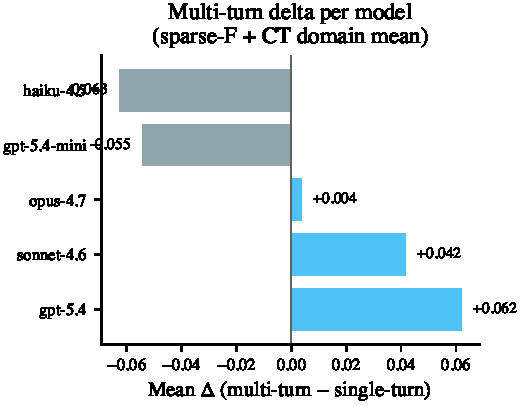
\includegraphics[width=0.55\linewidth]{figures/fig3_multiturn.pdf}
  \caption{Mean reward delta (multi-turn minus single-turn) per model
    averaged over sparse-Fourier and CT. Frontier models
    (Sonnet~4.6, GPT-5.4, Opus~4.7) gain; budget models (Haiku~4.5,
    GPT-5.4-mini) regress.}
  \label{fig:multiturn}
\end{figure}

\begin{figure}[!h]
  \centering
  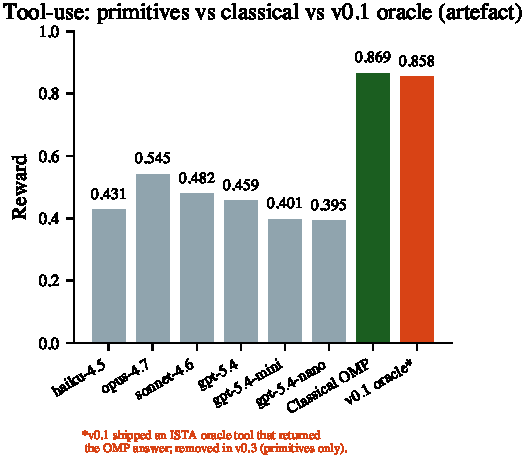
\includegraphics[width=0.55\linewidth]{figures/fig5_tools.pdf}
  \caption{Tool-use rewards on sparse Fourier recovery. v0.3 removed
    the \texttt{ista\_tool} oracle; tested LLMs (Haiku~4.5,
    GPT-5.4-mini) drop to the empty-answer floor, while classical
    OMP remains at $0.87$. The v0.1 oracle-artefact value ($0.858$)
    is shown for contrast.}
  \label{fig:tools}
\end{figure}

\end{document}
